%many ways in which the models of previous section would manifest: effects in
%- astrophysics (only way, if dark matter only interacts gravitationally)
%- particle physics (underground, fixed target, and colliders)

The interactions described in the previous chapter have many consequences in astrophysics (where they could modify the DM density) and in collider and non-collider particle physics experiments.% such as underground DD experiments, fixed target experiments and detectors at particle colliders, where non-gravitational interactions must play a role. 
%why colliders (what is a collider)
%- high energy
%- very well-understood detectors 
%- not able to prove non-interacting particles are invisible particles but
%- discover/study other mediators and other particles in dark sector, not just invisible particles
%why lhc (what is the LHC)
%- interactions may be feeble because because mediator is heavy, or because couplings to SM are small
%- highest energy, able to probe highest energy scales of any collider
%- largest luminosity for hadron-hadron collisions, can reach small couplings
%- complementarity: effective coupling to hadrons required for production in pp collisions, also required for nuclear scattering in DD

Collisions of known particles at high energy, observed with well-understood detectors, have been a very successful tool, leading to the discovery of many of the fundamental components of known matter in the SM. %link is completely missing here
While collider experiments alone cannot discover DM, they can discover invisible particles, and this could open up direct study of DM--SM mediators in other channels and additional particles of a dark sector. %this essentially means we are free from astroparticle uncertainties, more explicit?
DM--SM interactions may be feeble because they are mediated by a heavy mediator or by a mediator with small couplings to SM.
High energy and large numbers of collisions are needed to probe for these interactions, and the LHC, which presently collides protons at a center-of-mass energy of 13~TeV, will deliver both in the coming years. 
%The LHC, which presently collides protons at a center-of-mass energy of 13~TeV, is the highest-energy collider in operation.

Below we discuss experimental searches for invisible particles from three LHC experiments, ATLAS, CMS, and LHCb~\cite{ATLAS2008,CMS2008,LHC2008} and briefly touch on some results from previous colliders. %does ALICE search for invisible particles?
The LHC results include up to 36~\ifb of proton-proton data taken through 2017 during Run-2, more than three times what used for the Higgs discovery, but only 1\% of the data expected during the full High Luminosity (HL-LHC) run.

For signature, we outline how the relevant searches are done, some the challenges, and the information they provide on the properties of hypothetical particles (couplings, mediator mass, other parameters of the Lagrangian in a particular model). 
In a later chapter, we describe how collider information can be related to non-collider DM searches and to the present DM abundance, such as how conclusions drawn from relativistic collisions can be extrapolated to the non-relativistic collisions of DM+nucleons. 

\begin{marginnote}[]
\entry{Run-1}{First period of LHC running (2010-2012) at 7 and 8 TeV center-of-mass energy, where approximately 20~\ifb of data were collected by ATLAS and CMS.} %this is probably too much information
\entry{Run-2} {Second, ongoing period of LHC running (2015-2018) at 13 TeV center-of-mass energy, planning to collect approximately 100~\ifb of data.}
\entry{HL-LHC} {High-Luminosity LHC running period, planned to start in 2026 to collect 3000~\ifb.}
\end{marginnote}

%transition????
%We start describing searches for invisible particles interacting through SM bosons~\ref{sec:results_ZHSearches}, then move to generic searches for signals of invisible particles with missing transverse momentum and signals of mediators decaying into visible particles~\ref{sec:results_monoXSearches}, outline the searches for complete models with invisible particles candidates in Section~\ref{sec:results_SUSYSearches} and finally conclude with searches for long-lived particles~\ref{sec:results_LLPSearches}. Throughout this chapter
%and in Section~\ref{sec:experimentalChallenges} %CD: removed in favour of sidebars
%we will highlight the experimental challenges and the novel experimental techniques used to overcome them,
%motivated by the strong interest in dark matter searches. 
%We then conclude with searches for long-lived particles within models of invisible particles in
%Section~\ref{sec:results_LLPSearches}. %CD: need to rewrite this sentence, but the idea is: if we hadn't had invisible particles as a motivation motivation we wouldn't have done this difficult stuff. 

\subsection{Searches for invisible particles production mediated by SM-bosons}
\label{sec:results_ZHSearches}

%%%%Z TO INVISIBLE

%- we are sensitive to even lighter neutrinos than 1 MeV wimps
%- we have seen Z decays decay invisibly to light and weakly interacting particles: neutrinos
%-- how have we done that? a visible + MET search (with constraint, at LEP)
%- difference between invisible particles reactions in SM and new physics models: rates 
%- constrain with total Z to invisible
%- results (numbers)

%searching for invisible particles:
%The Z boson has a fuckload of invisible decays

%main background to many other searches for invisible 

%useless info about Z 
%CD only mentioning below because it's like a monophoton
%Simple (but somehow messy) explanation in https://cds.cern.ch/record/1750933/files/CERN-THESIS-2013-330.pdf, Hugo's student
%Hugo did it, unpublished: https://www-cdf.fnal.gov/physics/ewk/2007/ZnunuWidth/
%CDF direct: 466 pm 42
%\textbf{Decays of the Z boson into invisible particles} can be constrained using the invisible Z width. It can be measured directly in Z decays in association with a photon emitted as initial state radiation. Events are selected containing a single photon, missing transverse momentum and no other sizable event activity. This selection is also used for identifying events from possible invisible particles reactions at colliders.
%LEP combined: 503 $\pm$ 16 MeV
%The total Z width has been measured indirectly at LEP~\cite{ALEPH:2005ab} leading to a measurement of the number of light neutrino families compatible with cosmology; if the partial widths of the decays into visible particles are subtracted from the total width, the invisible width can be measured to 499.1 $\pm$ 1.5 MeV~\cite{Patrignani:2016xqp}. 
%The precision of the indirect measurement is better than that of the direct measurement, due to the higher statistics and the relative ease of selection and background subtraction for the visible Z decays. %CD: omitted, no space
%The main systematic uncertainty in this case comes from the theoretical uncertainties in the simulation. CD: Carena seems to think it is an uncertainty on fast simulation
%\begin{marginnote}[]
%Direct and indirect Z width measurements must agree if the decay of the Z to a pair of invisible new particles is to be the main mechanism responsible for the deviation from the SM values. 
%\end{marginnote}%CD: I think this is important to mention in the same sense as the caveats on the s-channel resonances, but it can be omitted
%in this case, an analysis of the mass of the system recoiling against the photon would provide a handle to distinguish between different BSM processes. %CD: omitted because this is possibly too handwavy but how can we summarize 4 pages of Carena in a sentence?
%Carena quantitative: At present, measurements at LEP and CHARM II are capable of constraining the left-handed Z\nu\nu-coupling, 0.45 <~ g_L <~ 0.5,  while the right-handed one is only mildly bounded, |g_R| <= 0.2.

For copious production of low-mass invisible particles, colliders already provide spectacular evidence: the huge rate of neutrino production mediated by the W and Z bosons. 
Neutrino production via the Z boson is often the largest background to searches for new invisible particles and is important to understand well.
The rate of would differ from the SM prediction if the Z boson is coupled to additional invisible particles lighter than about half its mass.
The most precise measurement of the invisible Z width, 499.1 $\pm$ 1.5 MeV, has been inferred from the total width at LEP~\cite{ALEPH:2005ab}.
%~\cite{Patrignani:2016xqp}
This can be used to constrain the parameters of models such as Z portals~\cite{Carena:2003aj,Escudero:2016gzx}.
%~Arcadi:2014lta,
The coupling between the Z and an invisible Dirac fermion is constrained to be smaller than 2-3\% for invisible particles that are significantly lighter than half the Z mass.
A less-precise direct measurement of the Z's invisible width, also by LEP, uses invisible decays with a photon emitted as initial state radiation (ISR), selecting events with a single photon, the total invisible transverse momentum inferred from momentum balance with the visible particles (\MET), and little other event activity.
This \MET+ISR has become a key signature for invisible particle searches at colliders. 
At the LHC, precision measurements continue to test the production and decay of Z bosons for the effects of invisible particles. 
For example, ATLAS has measured the ratio of cross sections for jet and \MET production, dominated by invisibly-decaying Z bosons, to production of Z bosons decaying to dilepton pairs, a ratio which is sensitive to the production of additional invisible particles~\cite{Aaboud:2017buf}. 

The Z boson is also key to invisible decays of the newly-discovered Higgs boson.
Higgs decays to neutrinos contribute to less than 0.1\% of its total decay width in the SM, proceeding through a pair of Z bosons that then both decay invisibly.
With present data, this rate could become observable if the Higgs is coupled to additional \IP~\cite{Khachatryan:2016vau,Aad:2015pla}.
%Englert:2011yb,
%% its small width to invisible particles in the SM is far below current experimental sensitivity, so an observation of invisibly-decaying Higgs would imply new physics. 
To constrain the invisible width of the Higgs, ATLAS and CMS cannot directly measure its total width in a model-independent fashion~\cite{Dobrescu:2012td}.
Searches instead attempt to directly observe these decays via their recoil against visible particles (substantial \MET), or by comparing measurements of the Higgs parameters under additional assumptions about the BSM physics.
Direct Higgs to invisible searches have used Run-1 and Run-2 data, combining several strong and electroweak production channels.
Combining direct and indirect searches, the most stringent bound on the fraction of invisible decays of the Higgs boson is 23\%~\cite{Khachatryan:2016whc,Aad:2015pla}.
This places constraints on Higgs portal couplings of 1-2\% for Dirac invisible particles much lighter than half the Higgs mass. 
%For the Higgs boson, the upper limit on the branching fraction to visible and/or invisible non-SM particles only using precision measurements is 34\%

\subsection{Generic searches for invisible particles from BSM mediation}
\label{sec:results_monoXSearches}

Searches for invisible decays via SM mediators (the Z or Higgs) can be viewed as special cases of searches for more general BSM mediation of invisible particles.
Since mediator decays to \IP are suppressed if the \IP mass is heavier than half the mediator mass, the fixed masses of SM mediators place a $\sim45$ --65~GeV upper bound on the \IP mass that can be observed.
Moreover, the distribution of \MET in such events has a similar shape to that of the Z-mediated neutrino background.
% and known properties of Higgs and Z bosons are exploited to reject backgrounds.

\begin{textbox}[!h]
\section{Measuring invisible particles: \MET reconstruction}

%10 words per line, 20 lines
%While at lepton colliders the initial center of mass energy is known and 
%can be used as an additional constrain to measure the momentum imbalance due to escaped invisible particles in the final state, measuring missing transverse momentum at hadron colliders
% TJ: Not sure why you make this distinction?
% I tend to think about the lepton collider case as offering
% one extra constraint, i.e. on the total missing *energy*
% but the directional MPT constraint still requires an
% inclusive measurement
Precise measurements throughout each detector systems are crucial to measure \MET in experiments at hadron colliders. This is because the calculation of \vec{\MET} should include all particles in the event.
% regardless of whether they are reconstructed as physics objects (jets, electrons...). 
Contributions that are not attributed to physics objects form the soft component of the \MET~\cite{Aad:2016nrq,CMS-PAS-JME-16-004}. 
One of the main challenges for \MET measurements are excluding contributions other than the hard-scatter process, e.g. from pile-up. 
Searches for invisible particles also need to efficiently reject events with large \MET if the visible energy is due to non-collision background. 

\textbf{Challenge: pile-up in \MET reconstruction.} 
%Momentum contributions from additional proton-proton interactions can have a significant contribution to the overall transverse momentum balance.
In addition to the pile-up suppression techniques applied at the calorimeter level, tracking information can be used to determine whether energy deposits originate from the primary collision vertex. 
The combination of this information is used to remove pile-up both in the physics objects used for \MET calculation and in the overall event energy balance~\cite{CMS-PAS-JME-16-004,ATLAS-CONF-2014-019}. 
%Trigger rates grow exponentially with the number of additional interactions

%[cite: https://cds.cern.ch/record/2205284/files/JME-16-004-pas.pdf, asked Emma and TJ for best reference]
%The lack of tracking information in the trigger system is a limiting factor in selecting events with low \MET at the trigger level, as the rates grow exponentially with the number of additional interactions. 
%from https://twiki.cern.ch/twiki/pub/AtlasPublic/MissingEtTriggerPublicResults/metxs_vs_mu.pdf

\textbf{Challenge: fake \MET rejection.} 
Non-collision backgrounds, such as cosmic rays, beam background and detector noise have a significant contribution to the tails of the \MET spectrum, as shown in Fig.~\ref{fig:fakeMET}
Specific quality cuts, based on the presence of tracks associated to the deposited energy and on energy deposited in the various calorimeter layers are applied to reject these events~\cite{ATLAS-CONF-2015-029}.~\footnote{The number of events passing the jet+\MET analysis selection before these quality cuts is about ten times larger than the SM contribution~\cite{Aaboud:2016tnv}.}. 
\end{textbox}

%Maybe move this to chapter 3

%\subsubsection{Missing transverse momentum}
%\label{sub:MET} 

%Main points:
%\begin{itemize}
%\item The measurement of \MET relies on the precise measurement of all reconstructed physics objects. 
%\item Some description of \MET significance may be needed, but it may also be too academic. 
%\item Fake \MET is rejected using quality cuts.  
%\item Pile-up needs specific techniques because of the soft terms. 
%\item \MET at the trigger level is the driving reason why we can't go lower, see next section.
%\end{itemize}

%from ooutline

%- Mismeasured MET (combining instrumental effects and beam/cosmics background)				
%	- CDF				
%		- beam background: exploit track pointing to jet and calorimeter layers				
%		- QCD: shitty method from Mario (extrapolation changing the veto)				
%	- LHC:				
%		- beam backgrounds: like CDF, more refined				
%			- can have a % of how many events would have been				
%		- QCD: matrix method a la SUSY				
%	- Other backgrounds (diboson, top)				
%		- Small so using MC				
%		- LHC has validation regions				
%			- check ttbar				

%Valerio's talk for relevant plots 
%https://indico.cern.ch/event/466934/contributions/2590281/attachments/1489278/2314178/20170706_EPS_invisible particlesatATLAS.pdf

%MET significance: in VBF CMS search
%For the 8 TeV dataset, an additional requirement is set on an approximate missing transverse energy significance variable S(Emiss) defined as the ratio of Emiss to the square root of the scalar sum of the transverse energy of all PF objects in the event [62]. Selected events are required to satisfy S(Emiss) > 4?GeV.

For heavier BSM mediators, this is not necessarily the case.
Their decay to invisible particles can produce \MET distributions substantially different than the SM background.
The complexity of the processes mediating invisible particle production determines the composition of the visible recoil, and so searches are employed across many different visible particle signatures. 
Nevertheless, many collider searches, from LEP to Tevatron to the most recent LHC searches (e.g.~\cite{Fox:2011fx,Bai:2010hh}), %Beltran:2010ww,
aim to be model-agnostic, designed to detect an excess of \MET over the SM background with minimal assumptions about the visible objects in the recoil.
Selecting events (triggering) in a model-agnostic way can often be done by looking for substantial \MET, but for models that do not produce large \MET, one is forced to assume more about the visible recoil.
We start with the 'jet+\MET' search, which illustrates techniques used in other general invisible particle searches, and shares with them many of the same challenges.
Traditionally, these have been called 'mono-X' searches, but the radiation of a single object is only the leading process in the simplest reactions~\cite{Haisch:2013ata}. 

%We begin this section by describing the LHC searches for missing transverse momentum in association with one or more hadronic jets. The jet+\MET search allows us to illustrate many of the techniques used in invisible particle searches, and it is one of the most powerful to constrain BSM-mediated simplified models of invisible particles. We then move on to outlining searches using different associated objects, and continue with searches for visible mediators that are the consequences of the invisible particles production mechanism. Finally, we compare and discuss the sensitivity of invisible invisible particles and visible mediator searches at the LHC. 
\begin{marginnote}[]
\entry{A \it trigger}{selects which LHC collisions are recorded for analysis. For descriptions of the ATLAS and CMS triggers, see ~\cite{Smith:2016vcs,Aaboud:2016leb,Khachatryan:2016bia}.}
\end{marginnote}

\subsubsection{Searches with jets}

%- searches for invisible particles (where the interaction is mediated by another particle) all have a common denominator in the large Z + (stuff) to invisible SM background
%- for H and Z we know signature is relatively low MET
%- with BSM mediators, we don't: looking in different slices of phase space (different MET regions) with different associated particles (different signal/background ratios and sensitivity to particular operators)

%Can think of searches for H->invisible and Z->invisible as tailored instances of more generic searches where mediator can be whatever the fuck. Invisible signals for masses above 45-60-ish GeV; up to half mediator mass. So: much wider range of the amount of MET is possible. So while the H-invisble searches are tailored to a particular range of mediator masses (90-125 GeV), a more generic set of searches, often termed 'mono-X' searches, are performed to probe this wider variety of signatures found in the BSM mediator models.

One way to reduce the model dependence of the searches is to require that the recoiling visible particles are produced by SM processes, not in the dark interaction.
ISR meets this criteria.
SM bosons are likely to be present in any BSM process, radiated from initial state partons at rates fixed by the SM.
Because gluon ISR is far more prevalent than the other forms, the jet+\MET search is a key search in this approach.% particularly when the details of the dark interaction are unspecified.

A jet+\MET search typically selects collision events with a moderate amount of \MET (in the 13 TeV analyses, typically above 200 GeV, sufficient to record such events at a manageable rate) and at least one jet with transverse momentum, \pt, larger than 100-200 GeV in the central region of the detector ($\eta<2.4$). 
From this sample, further restrictions on additional hadronic jets and other visible particles are used to suppress contributions from SM processes and from instrumental backgrounds causing spurious \MET.
These requirements reduce the generality of the analysis but also better isolate signal-like events.
For example, contributions from W bosons decaying to leptons are reduced by vetoing events with leptons, and top pair production is reduced by limiting the number of jets present.
The remaining SM multi-jet processes can exhibit large \MET when one or more jets is mismeasured.
Such mismeasurements often result in \MET along the axis of a jet, and this feature is used to reduce the background to about 1\% of the total.
%$\phi$ direction of the missing transverse momentum vector does not align with the direction of the four-momentum of the jets with the highest \pt (leading jets).
%The remaining QCD background estimated from data amounts to less than 1\% of the total background. 
Non-collision events (e.g., intersecting cosmic rays, beam-gas interactions, and calorimeter problems) can also produce spurious \MET events.
Fig.~\ref{fig:fakeMET} shows that such events dominates a high \MET data sample unless rejected with criteria tailored to the expected collision time and detector hardware.%Sidebar? Textbox?

After the above criteria, one arrives at a sample composed mainly of invisible decays of the Z boson (approximately 55-70\% of the total background).
%CMS excludes taus, while ATLAS does not. Too much detail imo. 
%numbers in Livia's talk: https://indico.cern.ch/event/682235/contributions/2817876/attachments/1576792/2490208/invisible particlesWG-2017_V2.pdf and in Francesca's talk:
%https://indico.cern.ch/event/682235/contributions/2817877/attachments/1576793/2490236/171218_atlas_ungaro.pdf
A substantial rate of semi-leptonic decays of the W boson also survives the lepton veto when the lepton is not reconstructed (approximately 20-35\% of the total background.

The main observable is typically the number of events in one or more \MET \textit{signal regions}, either exclusive (in bins of \MET) or inclusive (considering all events above a given \MET threshold). 
%with \pt $>$ 250 GeV (ATLAS) or \pt $>$ 100 GeV (CMS) and \MET $>$ 250 GeV (ATLAS) or \MET $>$ 200 GeV (CMS). 


%<<<<<<< HEAD
%Redundancy check
%\begin{marginnote}[]
%\entry{Trigger}{a detector system that decides which LHC collision events are to be recorded for physics analysis. For a description of the trigger systems of the ATLAS and CMS experiments, see ~\cite{Smith:2016vcs,Aaboud:2016leb,Khachatryan:2016bia}.}
%\end{marginnote}
%=======
%This selection ensures that all events with these characteristics are recorded by the trigger system for further analysis. Events with lower \MET suffer from higher instrumental and SM backgrounds, which prevents the whole event sample from being recorded due to storage limitations. 
%>>>>>>> e19a0a00062b30c8f27ae17ccf4962994f2e3aca

%Searches for invisible particles presents different challenges, depending on the invisible particle mass and boost. If the mediator is heavy, any light invisible particle will receive a boost and appear as an excess in the tails of the SM \MET distribution. If instead the invisible  particle pair originates from a light mediator, of the same mass range as the Higgs boson, it will manifest itself at low \MET. The low \MET suffers from a much higher rate of both instrumental and SM backgrounds.
%As a consequence, it is impossible to record and store all events with a low-\MET for further analysis, since at the data-taking stage (within the \textit{trigger} and data acquisition systems) it is difficult to obtain further handles to discriminate signal and background, and the sensitivity to low-\MET signals is compromised. This challenge will be discussed further for both visible and invisible particle searches in Sec.~\ref{sub:twoBody}.

\begin{marginnote}[]
\entry{Signal region}{a population of events enriched in contributions from signal processes. Data in this region are compared to SM predictions to search for new processes. }
%For example, a region with a high \MET and no other objects except for the ISR object is a signal region for a \MET+X search.
\entry{Control region}{a population depleted of signal contributions but with other characteristics close to the signal region. Control data are used to model or validate SM predictions.}
%For example, a region requiring no \MET and a process mimicking that of the signal region is a control region for a \MET+X search.
\end{marginnote}

%List of backgrounds & cut


\begin{figure}[!htpb]
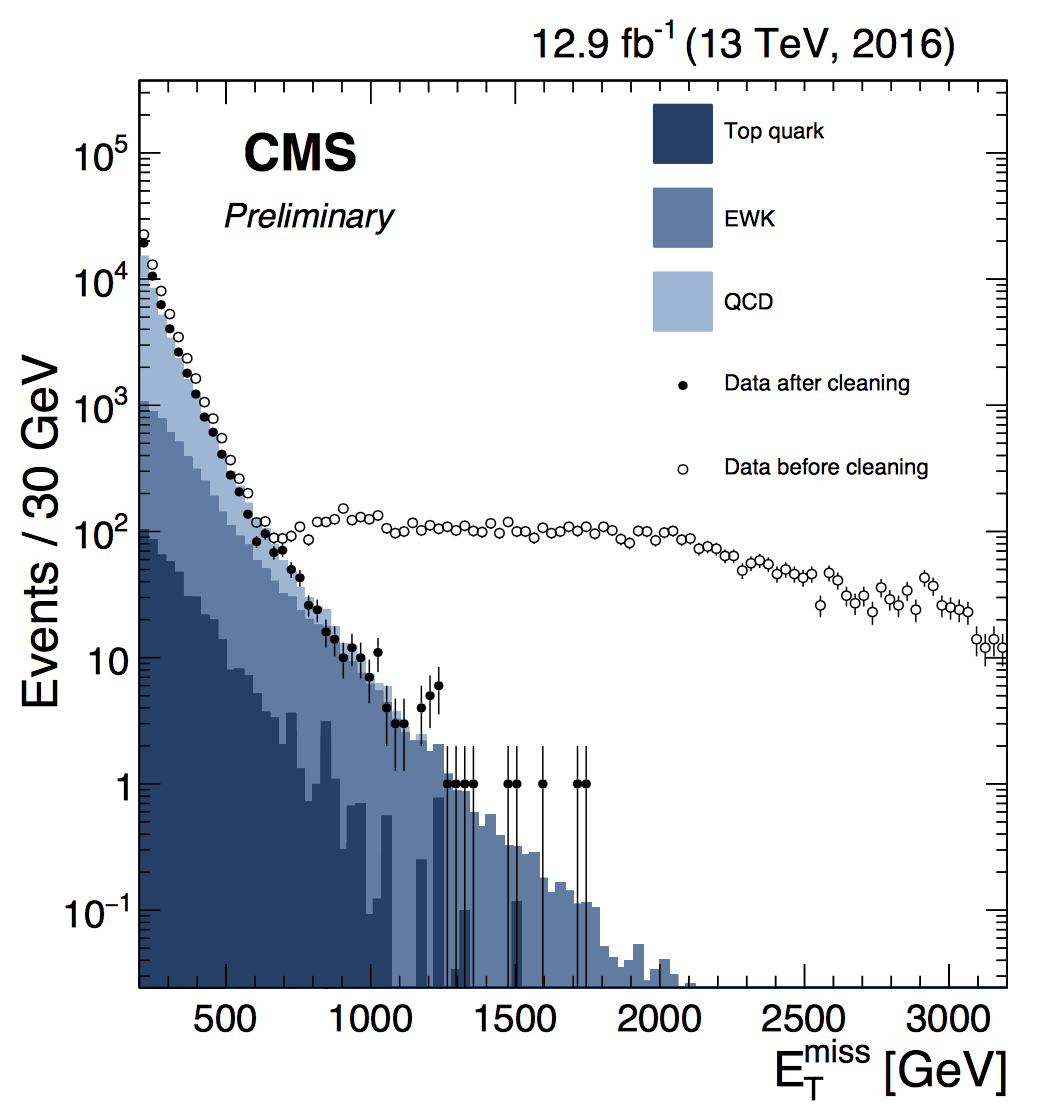
\includegraphics[width=0.5\textwidth]{figures/FakeMETTemp.png}
%Caption from the ATLAS monojet but they only have pT
%https://atlas.web.cern.ch/Atlas/GROUPS/PHYSICS/PAPERS/EXOT-2015-03/
\caption{The \MET distribution of events in a CMS \MET+jet search~\cite{CMS-PAS-JME-16-004}, selected for high total hadronic energy and at least two jets with \pt{} $>$ 400 and 200 GeV, before (open circles) and after (filled circles) rejecting spurious \MET backgrounds. The predictions of MC simulations (shaded) are also shown.
%data events passing the [define selection] without any cleaning criteria applied on the leading jet. The Standard Model background indicated in the plots corresponds to the estimates obtained for the analysis signal region, including jet quality requirements. 
%The jet selection inefficiency of the cleaning selection is O(1\%), which is negligible compared to the observed excess in data. 
Strong non-collision background suppression is vital to \MET+X analyses.}
\label{fig:fakeMET}
\end{figure}

%CMS: up to 4 leading jets 
%The CMS analysis also applies specific vetoes for photons and heavy flavour jets, to reject events with photon ISR or containing top quarks. The CMS analysis also includes a signal region targeting hadronic decays of the W and Z bosons using substructure techniques, which is considered separately in the case of ATLAS and will be discussed in Sec.~\ref{subsub:monoV}. 
%Estimating the background
%In order to reduce theoretical and experimental uncertainties on the main backgrounds, 
%
%big picture:
%- need a very precise estimate of the shape
%- calculations of this shape in QCD cannot be done to high enough order to get arbitrarily good precision
%- so predictions from available high order calculations are combined with data in the visible CR to blah.
%- combined means: use Zll as estimate of the shape, compare to MC, and correct for instrumental and other known effects.

Because \IP have feeble interactions with the colliding partons, and thus low production cross sections, these searches need very precises estimate of the shapes of the backgrounds.
%As an example, the integrated number of signal events with a \MET below 510 GeV amounts to less than 0.03\% of the background~\cite{Sirunyan:2017jix}. 
%>>> 162+130+98+85+65+53+54+41
%688
%>>> 136863+74340+42540+25316+15653+10092+8298+4906
%318008
%>>> 688./318008
%0.002163467585721114
A background estimate solely from MC simulation is subject to uncertainties on both theory and detector simulation affecting the total cross-sections and is therefore not precise enough.
To estimate the Z- and W-mediated neutrino backgrounds, recent ATLAS and CMS searches combine the information from data, in signal-free \textit{control regions} selecting visible boson+jet processes (W, Z, $\gamma$) and the most recent perturbative calculations~\cite{Lindert:2017olm}, much more precise estimates.
%The shape of the \MET distribution is taken from simulation, but its normalization is derived from data  
%where the transverse momentum of the visible decay products is subtracted from the total transverse momentum balance to obtain a proxy of the \MET distribution. 
%V+jet processes where the W and Z bosons decay into visible particles ($Z\rightarrow ll, W\rightarrow l\nu+jets$, where $l$ = $e, \mu$). 
%not sure we should say that the bin by bin estimates are used, here it's ambiguous
%The event selection follows that of the signal region, substituting a lepton requirement to the lepton veto in case of vector bosons. 
%[Consider adding more info about QCD/QED correction and importance thereof, citing Ellis's paper on UA1 discovery~\cite{Ellis:159861}].
%The estimation of the number of $Z\rightarrow \nu\nu$events from the $\gamma$+jet and  $W\rightarrow l\nu$+jets control region needs a specific treatment due to the difference in the processes. This is particularly important for a consistent treatment of the different processes used in the background estimation and of the main theoretical uncertainties. %CD: how do we call the thing
%The full information on the theoretical and experimental uncertainties and their correlations from this procedure is used in a simultaneous fit to control and signal regions, to determine the overall background estimate in each of the \MET regions considered. 
%and leads to an improvement of 40 to 50% in the search according to PhilHarris and Livia, but I wouldn't add that unreferenced
Backgrounds from top processes in ATLAS are estimated using a control region with $b-$jets, while CMS takes this background from simulation.
Estimates of smaller backgrounds rely more heavily on simulation.
%Smaller diboson backgrounds are estimated solely from simulation. 

%%Experimental uncertainties
To date, precision achieved for the background estimate is 2--7\% (CMS) and 2--10\% (ATLAS), depending on the \MET range.
The remaining uncertainties mainly arise from the identification of leptons (CMS) and the understanding of the jet and \MET calibration (ATLAS). 

%- our observable is the rate, then we convert that rate to the parameters of the model: couplings, given masses
%- model-independent as a function of MET cut
%- simplified models and Higgs portal
%  - couplings for different models
%  - Equally sensitive to 

%Model-independent
With no excesses observed, these searches can set 95\% CL limits on the production cross-section of invisible particles, typically spanning from 0.5\pb to 2\fb depending on the \MET threshold~\cite{Aaboud:2017phn}.
ATLAS and CMS also report constraints on a selection of mediator models.
These constraints can be interpreted as limits on the interactions between the mediator and the SM (e.g.\gq) under specific sets of model assumptions, not on the mass and other properties of the invisible particles per se.
As an example, for the simplified model with (axial-)vector mediators, mediator masses of up to 1.5--1.9~TeV~\cite{Aaboud:2017phn,Sirunyan:2017jix} are ruled out for an invisible coupling of \gdm=1. For lighter mediators than this bound, the search can exclude SM couplings of order 0.1, or alternatively lower \gdm values than unity.
With this amount of data, the searches are also becoming sensitive to lower-rate interactions mediated by (pseudo-)scalar mediators, and a recent ATLAS search~\cite{Aaboud:2017phn} sets explicit constraints on colored scalar mediators, where, for unit couplings and invisible particle masses of up to 100 GeV, the mass of the mediator is constrained to be above 1.7 TeV. 
Jet+\MET results from LHC Run-1 and the Tevatron have also reported constraints on EFT models.  

Since this type of searches can constrain a wider variety of interactions than explicitly considered, steps have been taken to allow easy reinterpretation of the results. 
ATLAS and CMS provide more detailed experimental results on the HEPData platform~\cite{Maguire:2017ypu}.
CMS also provides a simplified likelihood function encapsulating the result~\cite{Collaboration:2242860,Sirunyan:2017jix}.
%which under certain assumptions approximates the full likelihood using a reduced set of information, 
%and has been used for reinterpretation~\cite{Pobbe:2017wrj}.


\subsubsection{Searches with photons and vector bosons}
\label{subsub:monoV}
%monophoton, monoV

%What we wrote above
%One way to approach the [goal of model-agnosticism] is to require that the recoiling visible particles are produced by SM processes, not in the dark interaction. ISR meets this criteria. SM bosons are likely to be present in any BSM process, radiated from initial state partons at rates fixed by the SM. Because gluon ISR is far more prevalent than the other forms, the jet+\MET search is important particularly when the details of the dark interaction are unspecified.

%- many other searches with ISR+MET
%-- not the higher signal xsec
%-- interesting because they are lower xsec but also higher S/sqrt(B) 
%-- when the details of the dark interaction matter these can be enhanced (VVchichi) 
%-- even for a fixed model, if this is the subdominant channel, different (lower) trigger thresholds. looking for other ISR bosons or additional particles allows lower thresholds and more acceptance for signals 

%i like this part because motivation
Besides gluons, other particles can constitute visible-particle recoil.
In models where the recoil must arise from ISR, the rates for photon and electroweak boson radiation are much smaller than for gluon radiation.
Nevertheless, searches in \MET+photon and \MET+Z channels can play a complementary role alongside jet+\MET, with a smaller and different mix of backgrounds and different systematic uncertainties.
ATLAS and CMS have both performed searches in each channel.
With lower backgrounds, events can be recorded with lower kinematic thresholds, resulting in lower MET and visible \pt{} selections.
For example, the lowest \MET value probed by the Z+\MET search, where the Z decays into leptons~\cite{Sirunyan:2017qfc,Aaboud:2017bja}, is around 100 GeV, vs. 
200 GeV for the jet+\MET search~\cite{Sirunyan:2017jix}.

%this tells us about EFT and it's enough
These searches can play a much more powerful role when the recoil arises from the dark interaction itself rather than ISR.
In these cases, photon or vector boson recoil~\cite{Birkedal:2004xn,Petriello:2008pu,Carpenter:2012rg,Bell:2012rg}, rather than gluon recoil, may be the dominant signature.

% current song: https://open.spotify.com/track/11CTFD30oBVu5NPSgjLeyi. most of this album sounds like early 80's AC/DC
%i don't know this album enough
%i'm on "love and affection" soon catching up
In these searches, the event selection and the background estimation strategies generally mirror those of the jet+\MET search, but vary with the type of recoil, taking advantage of the special features of the signal.
In the photon+\MET searches~\cite{Aaboud:2017dor,CMS-PAS-EXO-16-014}, components of hadronic showers mis-identified as isolated photons are a sizable background to be rejected.
The searches with electroweak bosons decaying hadronically use jet substructure techniques~\cite{Sirunyan:2017jix,Aaboud:2016qgg} to recover information about boson mass and decay in events where the decay products from the high-\pt{} boson are collimated.
QCD jets will not present any substructure~\cite{Larkoski:2017jix}, while the decay products of vector bosons grouped into large-radius jets have a typical two-prong pattern from the hadronization of the quark-antiquark pair.

None of these searches yet observes a signal. The searches are not in general as sensitive as the jet+\MET search to models where the visible recoil arises from ISR, because of smaller signal acceptance and comparable signal to background ratio, but they can be remarkably competitive---after the jet+\MET searches, the photon+\MET searches are the next-to-most powerful probe.
%, with 95\% CL cross-section limit on invisible particle production constrained to be below 2.5 and 7~\fb depending on the \MET threshold~\cite{Aaboud:2017dor} ranging from 150 to 300 GeV, as opposed to numbers that are not comparable because they are for a different cross section / process.
However, these searches provide the most stringent limits on some models where the boson in question is directly involved in the dark interaction~\cite{Petrov:2013nia,Berlin:2014cfa}.% excluding EFT scales between 150 and 750 GeV for \mdm=100 GeV, assuming the maximal coupling value allowed by perturbativity.

\subsubsection{Search signatures including the Higgs boson}

% what we wrote above Besides the gluon, other particles can constitute the visible-particle recoil against invisible particle production. In the model-agnostic case discussed above, where the recoil arises from ISR, the rates for photon and electroweak boson radiation are much smaller than for gluon radiation

%- old to new: 
%- why we are so keen on doing monohiggs searches:
%
%-- because if DM couples to the Higgs this is the only way to see it 
%--- actually not because monojet in lagrangian too

%- study of higgs properties is a big focus of ATLAS and CMS
%- looking at the higgs in lots of ways
%-how we do Higgs searches: 
%-- like we did before, depending on the decay product, then we stick MET in it and kill backgrounds even further
%-- complementarity between bbar and gammagamma in the same way as before

One can also look for the newly-discovered Higgs boson in the recoil, but due to the heavy mass of the Higgs and the small heavy-flavor content of the proton, the rate of Higgs ISR is insignificant. 
Thus, searches for \MET+Higgs target dark interactions in which the Higgs is a direct participant, and therefore the interaction is closely tied to the Higgs sector. 
This is a feature of many models that extend the SM scalar sector, as described in Sec.~\cite{sec:BSMMediatorModels}. 

Dedicated searches for \MET+Higgs select Higgs events similar to the inclusive Higgs measurements, then require substantial \MET to reduce the backgrounds to the search.
In the Run-2 data, searches in the $H \rightarrow \gamma\gamma$~\cite{CMS-PAS-EXO-16-054,Aaboud:2017uak} and $H \rightarrow b\bar{b}$~\cite{Aaboud:2017yqz} channels have been performed.
%why these channels and not the others
%we could use ZZ but it's not out yet not enough events really even with no ?MET
% other options are: WW and ZZ. these involve lots of additional complications. WW has a lot of different backgrounds, and ZZ is s
%do we say that? no space? i have "due to their relative experimental simplicity and/or high rates"
Searches in the $ZZ, WW$ and $\tau\tau$ channels are expected to contribute as well, once substantially more data is collected. 

% results / challenges
The \MET+$H \rightarrow \gamma\gamma$ searches~\cite{CMS-PAS-EXO-16-054,Aaboud:2017uak} benefit from their ability to precisely constrain the diphoton pair to the Higgs boson mass.
They are still statistically-limited.
The relatively low backgrounds allow probing for anomalous \MET as low as 50 GeV~\cite{CMS-PAS-EXO-16-054} .
The diphoton invariant mass is fitted in different signal categories, each optimized for different types of signal models. . 
%The SM background is estimated using a fit to the diphoton mass distribution, in events categorized
%according to their missing transverse momentum for CMS (50$<$\MET$<$130 GeV and \MET$>130$ GeV)
%or according to specifications optimised for different signal categories.%this is useless but the analysis is needlessly complicated  
The search for Higgs decays to two bottom quarks~\cite{Aaboud:2017yqz} requires \MET$>$150 GeV. All backgrounds except for the QCD background are estimated using MC simulation and constrained in dedicated control regions. 
It also employs jet substructure techniques for \MET$>$500 GeV to select boosted Higgs decays from a background of QCD processes.
The main systematic uncertainty for the lower \MET signal region is the modelling of the V+jets background, while higher \MET signal region is still statistically limited with the current dataset.

Absent signal, limits are set on the baryonic Higgs benchmark model outlined in Sec.~\ref{sub:simplifiedModels} with  \gq=1, \gdm=1, \ghZprimeZprime/$m_{Z}$=1, \sinthetab=0.3, 
%CMS: mZ'=10-10000 GeV, minvisible particles=1-1000 GeV
%CD: it would be nice to say what this can be reinterpreted to but we have no space
and on a Z'-2HDM models~\footnote{ In the case of the Z'-2HDM particles model, CMS and ATLAS set different masses for the new Higgs bosons, 
%https://docs.google.com/presentation/d/10R9XJaoMDEhXKhd_Wx9yMXEaPl4uXR8IcmuTeLancvg/edit#slide=id.g1f308da957_0_17
%ATLAS fixes both to 300 GeV, CMS fixes to mA0 
%For the record:
%CMS: A and Z' varied between 300-800 and 600-2500 GeV respectively
%ATLAS: mZ? = 400 to 1400 GeV, mA0 = 200 to 450 GeV
%The masses of the neutral CP-even scalar (H0) and the charged scalars (H�) from Z?-2Hinvisible particles model are set to 300 GeV. The invisible particles mass m? is set to 100 GeV 
%CMS: 
%Two-Higgs-doublet-Z' signals with a pseudoscalar mass of 300 GeV are excluded at 95\% CL for Z' masses below 900 GeV
%Baryonic Z' models with a invisible particles mass of 1 GeV are excluded at 95% CL for Z' masses below 800 GeV
so the constraints are not yet directly comparable.}.

Higgs+\MET and Z+\MET searches are also sensitive to extended scalar sectors such as two Higgs doublets with a scalar or pseudoscalar mediator~\cite{Bauer:2017ota,Ipek:2014gua,No:2015xqa,Goncalves:2016iyg,Bell:2016ekl}.

% with $tan\beta$=1, \gZPrime=0.8 and \mdm=100 GeV
%this is a dump, too long? i can't quite see how to make parallels between the two searches as they are really different

\subsubsection{Searches with third-generation quarks}
%ttbar+MET
%reinterpretation of SUSY

%- what is important 
%-- one step beyond ISR searches: search for a specific production, constrains to be a specific type of model. 
%-- once we know what we're looking for, we can look more effectively
%-- more stuff: more jets + more specific (b jets not any old shit)
%-- add heavy flavour jets produced in association with the MET (coming either from mediator or from production)
%- aha it was susy all along
%- results on scalar and pseudoscalar: is it better than monojet?

%Generic searches employing one single additional type of object produced in association with \MET are powerful tools to probe simple models of invisible particles. 
% More complex models, however, bring more handles for discovery: steps in this direction can be taken with searches using 
In scalar- and pseudo-scalar-mediated simplified models, one can exploit the production mechanism in the search design. For instance, the mediator can be produced along with two top or bottom quarks, leading to a signature of \MET and multiple b-jets.

A recent ATLAS search in these channel~\cite{Aaboud:2017rzf} is optimized for both recoil consisting of semileptonic and fully hadronic top quark decays and recoil with one or two bottom quarks.
This signature is similar to that of third-generation quark superpartners and can be part of dedicated SUSY searches or used for reinterpretation~\cite{Aaboud:2017aeu,Sirunyan:2017leh}.
SUSY searches suppress most of the $t\bar{t}$ background, matching specific models to specific, low-background signal regions. 
Relative to these approaches, the search in Ref.~\cite{Aaboud:2017rzf} is less narrowly targeted at specific models, where control regions can be more reliably developed, instead relying more heavily on simulation.
The sensitivity of searches of \MET associated to top quarks is comparable for the two strategies. 

No excess is observed in any of these searches. 
For \IP masses of 1 GeV, color-neutral pseudo-scalar mediators of mass 20-50 GeV~\cite{Aaboud:2017aeu} and scalar mediators of masses up to 100 GeV~\cite{Sirunyan:2017leh} are excluded. %CD: it would be nice to find out why this difference in sensitivity? 
%The increased LHC dataset will allow these searches to be sensitive for other invisible particles masses. 
Signatures with $b\bar{b}$ pairs are less sensitive to models that do not explicitly privilege bottom quarks, but can set much higher limits on colored mediator masses in case of preferential couplings to bottom quarks~\cite{Agrawal:2014una}. 

%for invisible particle masses of 35 GeV and couplings corresponding to the , the lower limit on the scalar  
%if limits of about 1 TeV on the masses of colored scalar mediators coupling explicitly to bottom quarks~\cite{Agrawal:2014una} for invisible particle masses of 35 GeV.   
%Mediator masses for the b-flavored colored scalar 
%model discussed in~\cite{Agrawal:2014una} are excluded up to 1.1 TeV for invisible particles masses of 35 GeV. 

%Not spending more than one sentence on monotop, is that ok?
Other LHC searches in this category are those only including only one top or bottom quark (also called mono-top or mono-bottom searches)~\cite{Sirunyan:2018gka, Aad:2014wza}.
They place constraints on models that include singly-produced invisible particles candidates through flavor-changing neutral currents~\cite{Boucheneb:2014wza}.

%scalar and pseudoscalar mediators decaying into invisible particles (including the case of colored scalars), 
%The CMS search uses substructure techniques to identify events with boosted top quarks. 

%In SUSY-like searches, the dominant $t\bar{t}$ backgrounds
%are heavily suppressed using variables that combine visible and invisible
%mass~\cite{Lester:1999tx} targeting the model sought. 
%This step uses information that is model-dependent,
%but increases the sensitivity to specific processes. The remaining
%small backgrounds are estimated using simulation. 

%The dominant backgrounds in~\cite{Aaboud:2017rzf} are estimated separately
%using MC in each of the signal regions,
%and their normalization constrained using control regions in a simultaneous fit.
%The main uncertainties for these searches are, depending on the signal region, 
%theoretical and MC simulation related uncertainties, jet energy scale and resolution. 
%and uncertainties related to the identification of heavy flavor quarks. 

%The main backgrounds for these searches are single top or misidentified $t\bar{t}$ processes. 
%The search where the top quark decays hadronically
%employs substructure techniques to tag the boosted top quark decays.  
%These searches place constraints on models of invisible particles (resonant, non-resonant). 

\subsection{Searches for SUSY invisible particles}
\label{sec:results_SUSYSearches}

%%SUSY results, generic

%Good talk for ATLAS:
%http://cds.cern.ch/record/2299118/files/ATL-PHYS-SLIDE-2017-1008.pdf
%SUSY2017 summary
%https://indico.cern.ch/event/695201/contributions/2853913/attachments/1582877/2502678/011618_SUSY17Summary.pdf

%First establish that Z and H don't have a ton of decays in invisible particles. Then they become background. 
%We see tons of events in monojets. They are all background. 
%Next searches: reduce rates but also background by asking for additional objects.
%SUSY many additional objects (search for gluino etc because the neutralino is guaranteed) 
%LLP look for weird additional objects that give you background rejection in case of very very rare stuff like dark photon it is the only wayyyyyyyyy.

 
%- overview of what SUSY searches are like and how they fit in
%-- so we know more about the specific final states and we can target them
%-- cost: many searches so we can't describe them all, broad strokes
%-- before we had minimal number of ingredients, so forced to exploit SM handles
%-- now we have a full copy of the SM that we can use, 
%- 

%transitions: 

%- searching for decay chains of specific superpartners ending in neutralinos gives strategies to reject background
%- one more step towards full models, know more about the final state so we target it

So far, motivated by simple models, the \MET+X experimental searches discussed make few choices about the visible recoil particles, i.e. the species of a single particle, yet these already lead to a plethora of diverse signatures.

Models with more degrees of freedom may vastly expand the set of signatures to be explored.
Supersymmetry (SUSY) adds, along with invisible particles, many more ingredients: a full copy of the SM particle spectrum.
Each superpartner features particular decay chains that can be targeted to a greater or lesser degree, privileging either generality or maximal sensitivity. 
Compared to the generic searches above, SUSY searches general opt for a more specific decay topology and thus apply more stringent event selections based on the expected kinematic features, often using discriminating variables based on a combined mass of visible and invisible particles (see e.g.~\cite{Lester:1999tx}) to recover the ability to resolve various resonant decays.

SUSY has received much attention by ATLAS and CMS, and many searches for its particles, such as for squarks and gluinos, have a long history at earlier coliders as well.
In this section, we give a flavor of experimental results of more recent interest.
%, concentrating on those that specifically highlight the connections to cosmological observables. 

%Removed fig because takes up space and it's easy to read
%\begin{figure}[!htpb]
%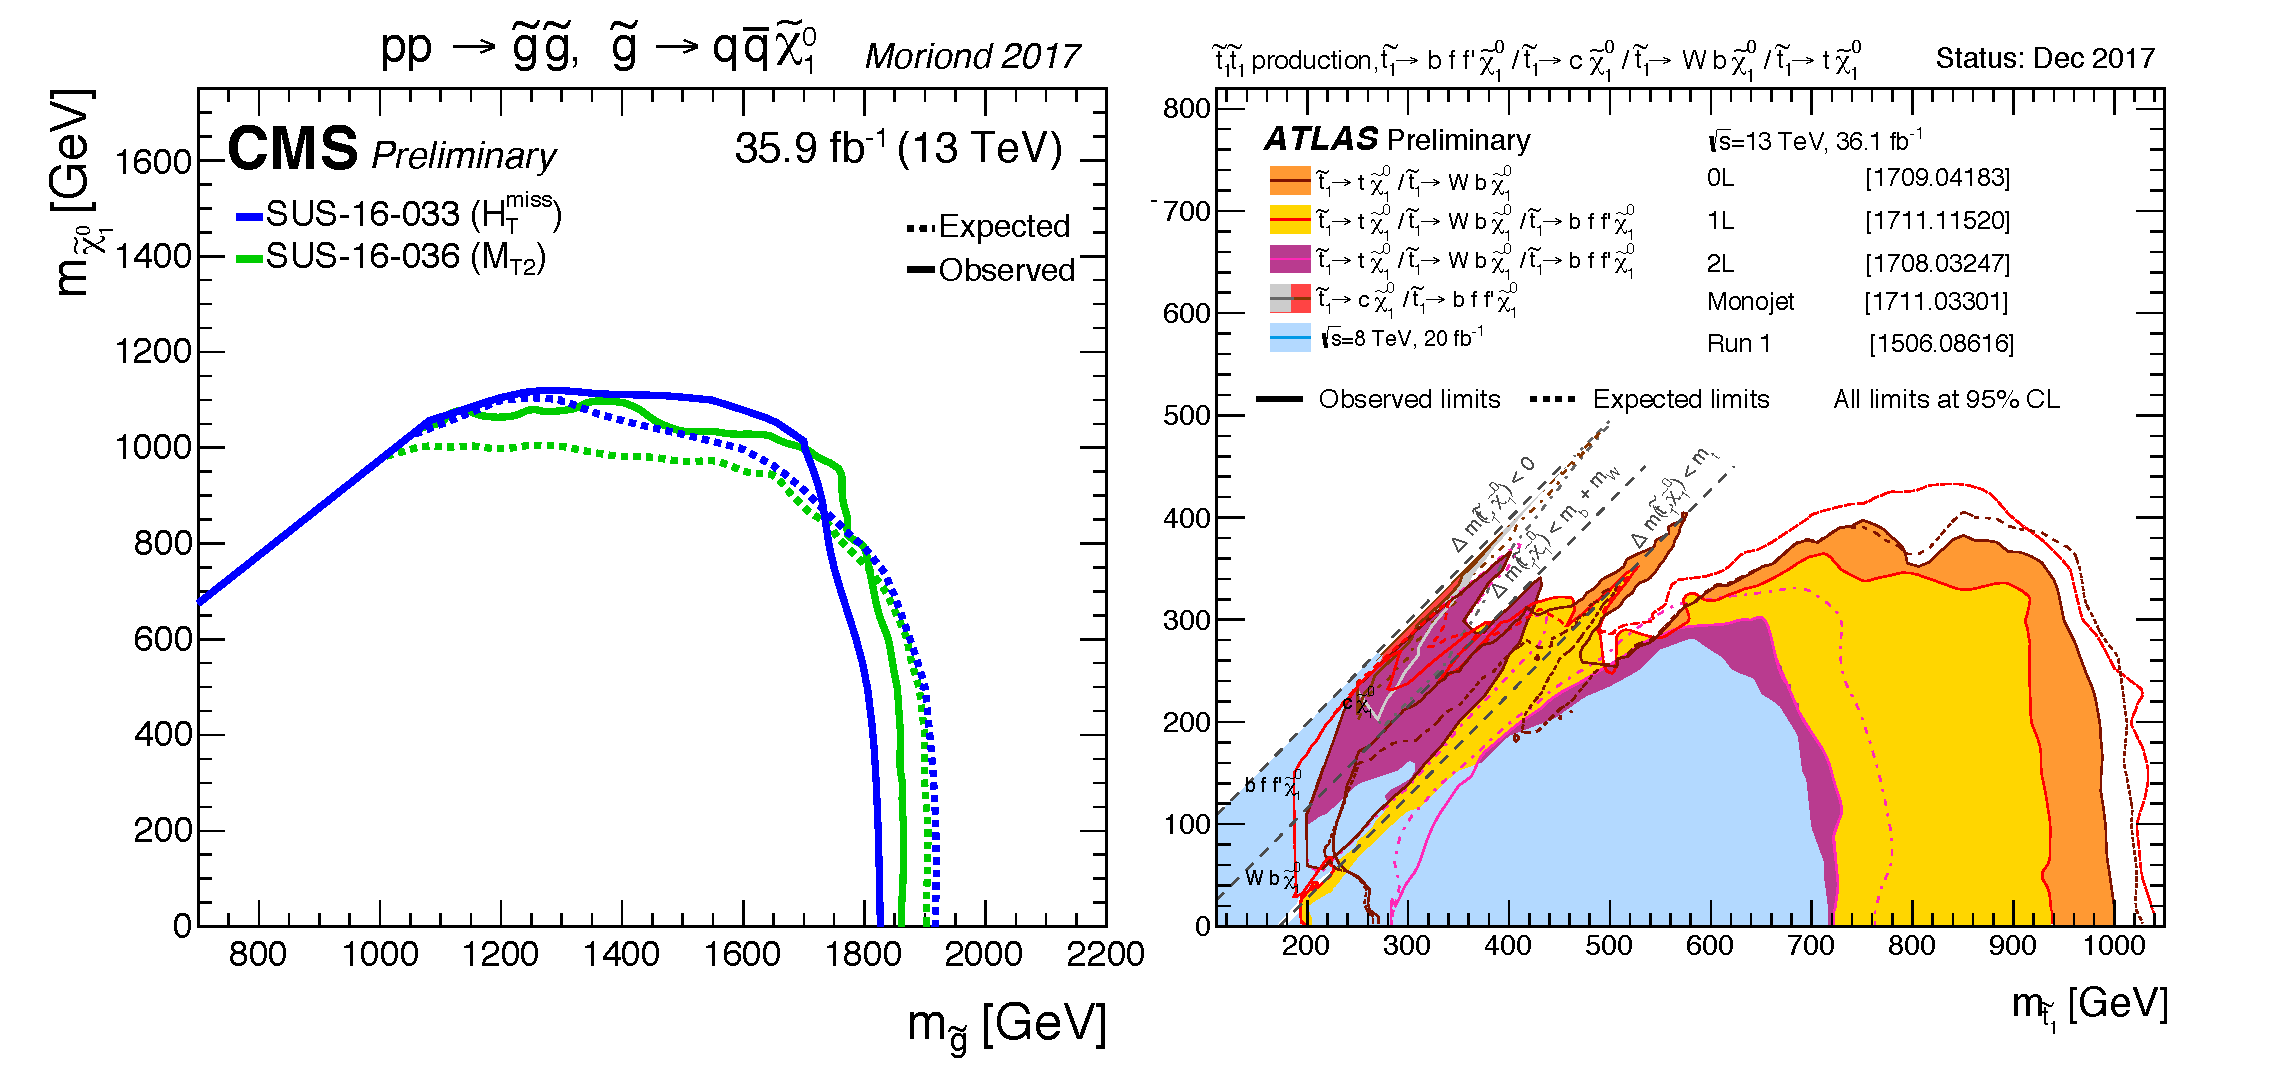
\includegraphics[width=\textwidth]{figures/SUSY_strong_ttbar.pdf}
%\caption{Mass reach of ATLAS and CMS searches for a selection of results targeting strongly produced SUSY particles, available as of December 2017. From~\cite{ATLASSUSYSummary,CMSSUSYSummary}.\label{fig:SUSYSummary_strong}}
%\end{figure}

No SUSY search so far has produced a conclusive signal. However, given its multifarious signatures, it's difficult to make general statements about the current status, even for simplified models of SUSY. Perhaps the best one can say is that searches for strongly-produced superpartners constrain them for masses approaching a couple of TeV (see Fig.~\ref{fig:SUSYSummary_ew} and e.g.~\cite{Aaboud:2017bac,Sirunyan:2017yse}), for neutralino masses up to a TeV, and,
%https://twiki.cern.ch/twiki/pub/CMSPublic/PhysicsResultsSUS/T1tttt_limits_summary_cms_Moriond17.pdf
on the other hand, other processes are less constrained.
Direct production of weakly-coupled superpartners has a much smaller production rate, and hence the constraints on them are significantly weaker.
Third-generation squarks are generally only constrained to be at least several hundred GeV for neutralinos of similar masses, see e.g.~\cite{Sirunyan:2017wif,Aaboud:2016wna}.
% and Fig.~\ref{fig:SUSYSummary_strong}. 
%https://atlas.web.cern.ch/Atlas/GROUPS/PHYSICS/CombinedSummaryPlots/SUSY/ATLAS_SUSY_Stop_tLSP/ATLAS_SUSY_Stop_tLSP.png
%https://twiki.cern.ch/twiki/pub/CMSPublic/PhysicsResultsSUS/T2tt_limits_summary_cms_Moriond17.pdf
But there are numerous exceptions to these blanket statements, even before one remembers that the masses exclusions shown in the figure only apply to specific slices of a multi-dimensional model parameter space.

\begin{figure}[!htpb]
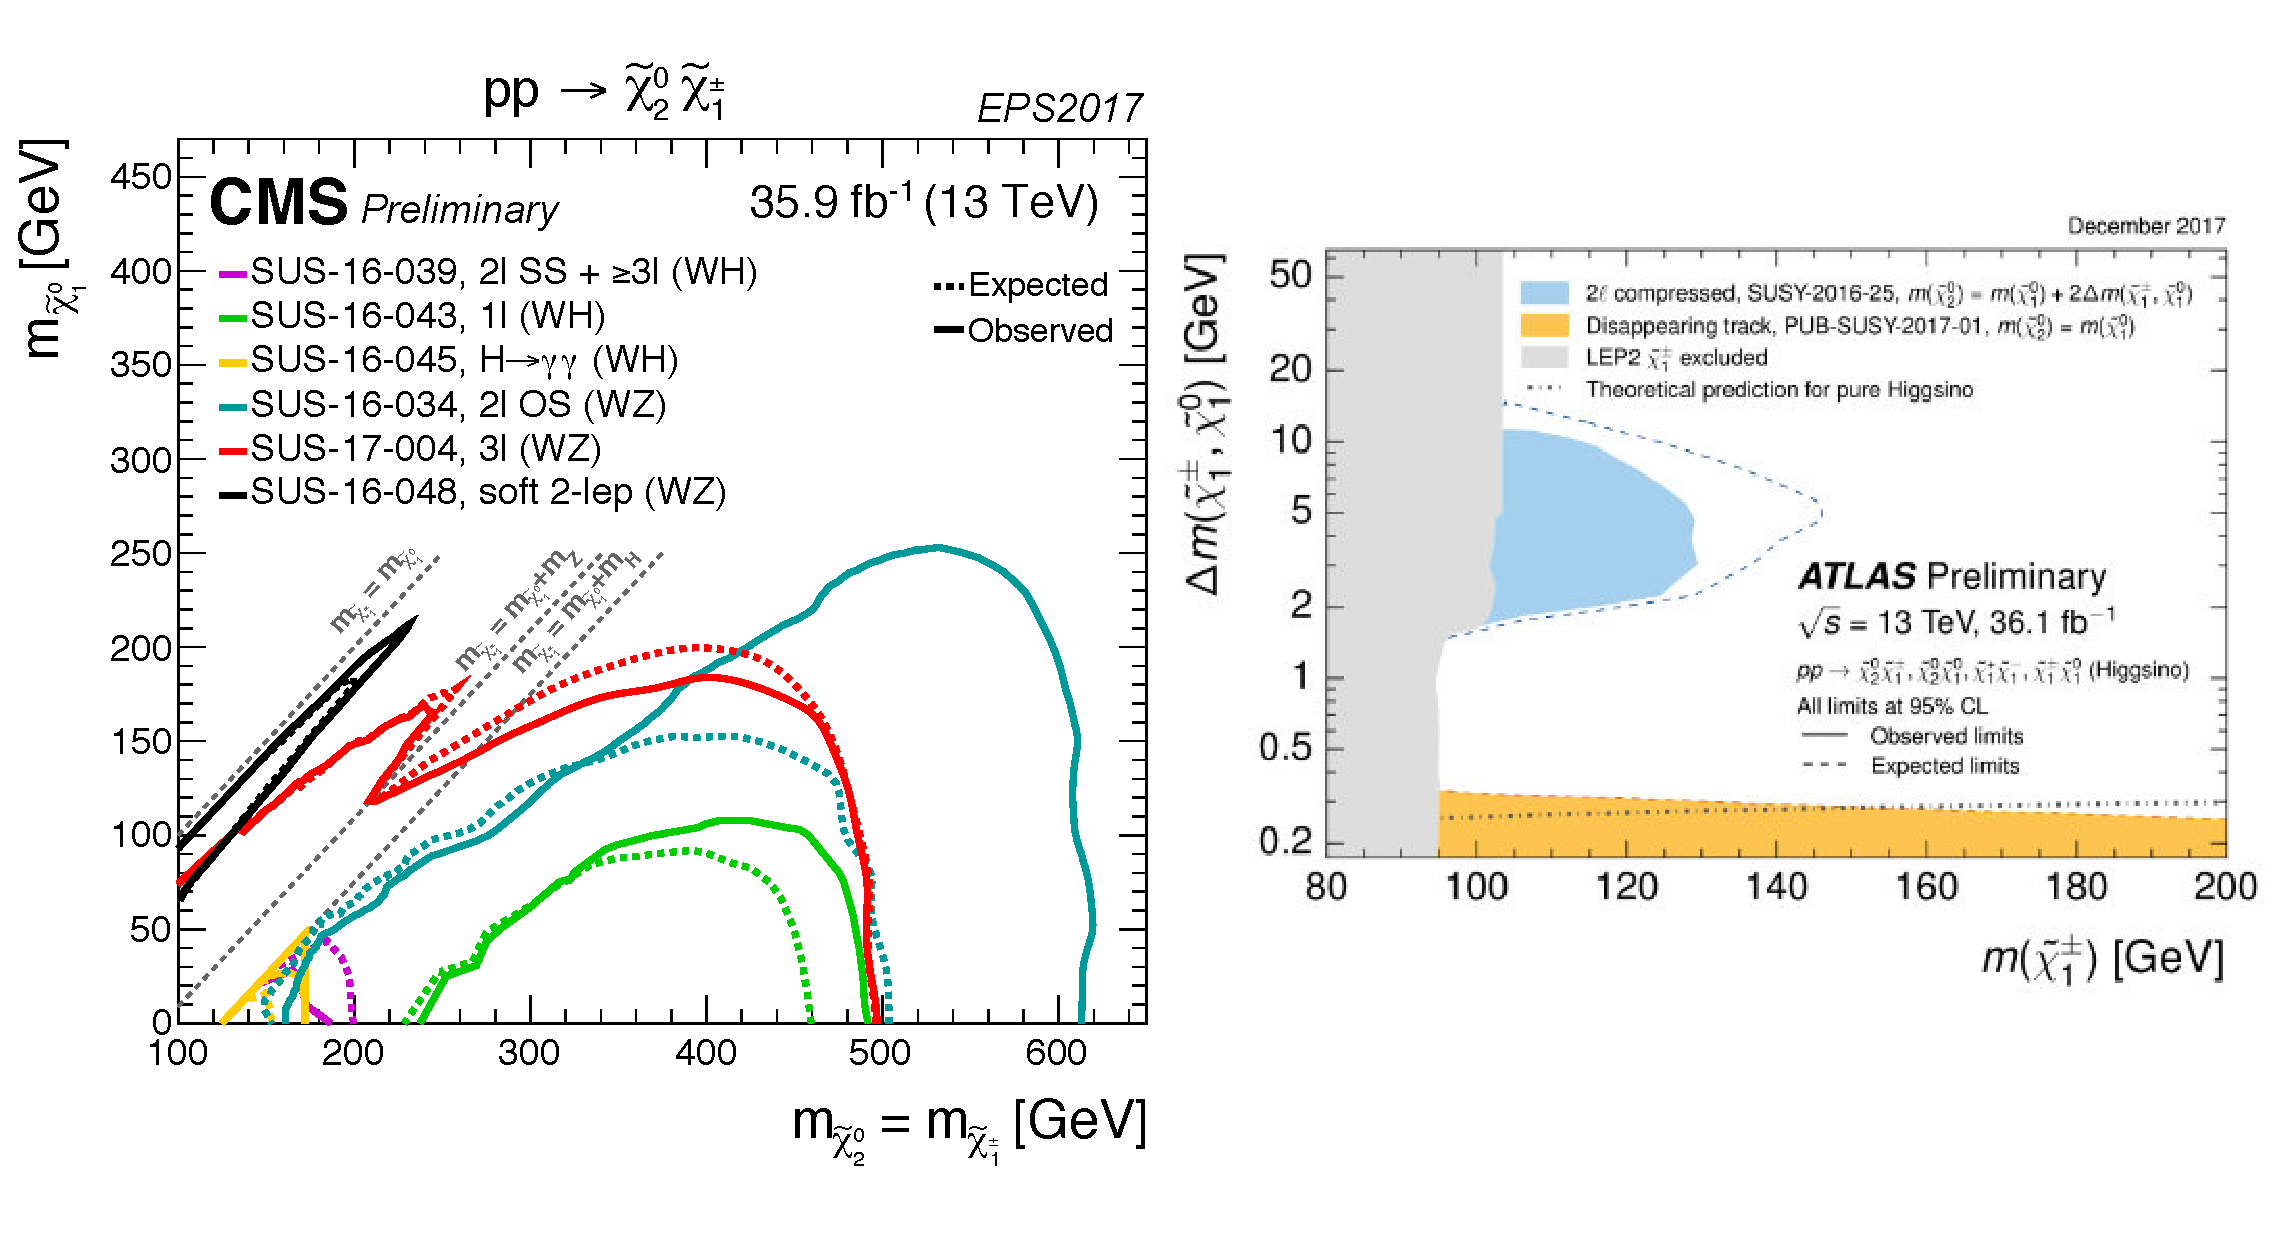
\includegraphics[width=\textwidth]{figures/SUSY_electroweak.pdf}
\caption{Mass reach of ATLAS and CMS searches for a selection of results targeting electroweak SUSY production, available as of December 2017. From~\cite{ATLASSUSYSummary,CMSSUSYSummary}.\label{fig:SUSYSummary_ew}}
\end{figure}

%https://atlas.web.cern.ch/Atlas/GROUPS/PHYSICS/CombinedSummaryPlots/SUSY/ATLAS_SUSY_EWSummary/ATLAS_SUSY_EWSummary.png

Though LHC searches have mainly probed strongly-produced SUSY channels so far, searches for rare processes are now entering their prime.
With the data now collected, one can explore the electroweakino parameter space (see e.g.~\cite{Sirunyan:2018ubx,ATLAS:2017uun}). %, by combining several channels as in
Searches for gauge boson superpartners (gauginos) can reach approximately 1 TeV if the superpartners of SM leptons are light, and the search can benefit from a high leptonic branching ratio, whereas their reach is lower if their decays proceed through W and Z bosons. %can reach 600 GeV 
More luminosity also provides access to new regions of parameter space for specific signatures, e.g. ``compressed'' regions where small mass differences between superpartners lead the signals to lie buried in large backgrounds at low \MET~\cite{Aaboud:2017leg,Sirunyan:2017zss}.
Small mass differences can also suppress superpartner decays, resulting in long lifetimes. This can be exploited to study regions with a mass difference as low as 0.2 GeV for Higgsino models~\cite{ATL-PHYS-PUB-2017-019}.
Other mechanisms of decay suppression can do this as well (e.g. split SUSY~\cite{Sirunyan:2018vjp}). 

%%SUSY scans
%% Targeting a specific signature, such as a cascade decay in a specific simplified SUSY model, improves the ability to discover it. A narrower focus however trades generality for sensitivity, especially when interpreting results in terms of simplified models. 
%Designing and interpreting searches solely using simplified models may not capture the spectrum of possibilities
%given by full, theoretically well motivated models. 

Despite the unwieldy diversity SUSY signatures, a sufficiently specific model can provide a concrete framework on which to build an understanding of the combined effect of many experimental constraints. Ref.\cite{Conley:2010du}, continued in LHC experiments ~\cite{Aad:2015baa, Khachatryan:2016nvf}, uses the pMSSM to define a finite (though large) parameter space for whichthe  wealth of experimental constraints can be systematically evaluated.
Though this approach is not exhaustive, it can identify under-examined signatures for future emphasis.
Besides particle physics data, one may also identify the LSP with astrophysical DM to focus more specifically on regions compatible with a given cosmology, as in Ref.~\cite{Aaboud:2016wna}.
 %this is EW dark matter interpretations of ATLAS, maybe leave for comparisons section?

%Many tools (e.g. ) need to be combined to obtain these parameter scans. 
Collaborations such as GAMBIT~\cite{Athron:2017ard} and Mastercode~\cite{Bagnaschi:2017tru} have combined a variety of tools to aid in such efforts.
These codes encapsulate search results in statistical outputs which can be combined to construct global constraints for the models of interest. 
For example, one may compile the likelihood functions for the parameters of a SUSY model given the results from collider, direct, and indirect detection experiments.

\subsection{Searches in association with long-lived particles}
\label{sec:results_LLPSearches}

%unconventional reconstruction techniques
%- more eLLP phase space
%- disappearing tracks
%- compressed SUSY
%- dark boson models that are light because haven't seen heavy
%- detector signatures of dark bosons
%- dark photons
%- LHCb

%extreme range of experimental objects
% So far, we've only discussed signatures of invisible particle production where the 
Prompt decays produce visible recoil originating at the collision point, and thus it can be reconstructed using the techniques for which the experiments were designed.
The long-lived mediators described in Chapter~\ref{sec:LLPModels} present different experimental challenges. 
For short lifetimes, long-lived particles (LLPs) can decay inside the tracking detectors, appearing as displaced decay vertices. 
%need citation
Some SUSY decay chains lead to disappearing tracks, if the visible particles decay into the LSP and soft particles (see e.g.~\cite{Aaboud:2017mpt, CMS:2014gxa}). %(e.g. in split supersymmetry) 
%Another distinctive experimental signature of LLP is the "disappearing track", produced for example by SUSY models where a chargino
%with a short lifetime leaves a track in the inner detector which effectively disappears as it decays into a neutralino and a soft pion~\cite{Aaboud:2017mpt}. 
%disappearing track ATLAS
Even longer-lived particles can decay in the calorimeters or in the muon spectrometers
%need citation
or they may even exit the detector cavern completely before decaying. 
%need citation
These complications add yet another dimension of complexity to such searches, because observing the events may require dedicated triggers, reconstruction algorithms, and even detectors\cite{Ball:2016zrp,Chou:2016lxi}. 
%Nevertheless, these searches motivate specific, time-consuming detector and algorithms improvements, given that LHC searches didn't find any prompt new physics yet and given our ignorance of the dark sector and its interactions. 
%backgrounds generally small and instrumental (no SM), but difficult searches

%Besides LLPs in SUSY, there is a class of search  to very light dark vector and scalar bosons.% and their connection to the generic searches for prompt, high-mass vector and scalar mediators. -> this is something that goes in future

%summary diagram in https://indico.cern.ch/event/656211/contributions/2673379/attachments/1498650/2333150/UW_dark_photons.pdf

% don't know where this goes
%The LHC searches mentioned in this chapter, with the exception of compressed SUSY scenarios, 
%so far target prompt production of WIMP invisible particles or associated mediator particles at colliders. 
%The absence of a signal constrains these traditional WIMP models to have small cross-sections and high mass scales. 
%This is one of the reasons why less-accessible dark boson and dark scalar models, including mediators with masses from the MeV to the tens
%of GeV and with a range of potential lifetimes, are a target that is gaining interest by LHC searches. A similar consideration
%applies for SUSY scenarios that are hard to detect. 
%These signatures are particularly challenging for ATLAS and CMS, given that many of these possibilities escape
%conventional detection.

Searches at colliders use a variety of experimental signatures to target different types of dark bosons, such as dark vector or scalar bosons.
%Is it produced in DY collisions
An LHCb search for dimuon resonances~\cite{Aaij:2017rft} is sensitive to visible decays of vector mediators in the mass range between 10 and 70 GeV.%, avoiding the regions with SM resonances decaying to dimuons. 
This search can use the entire sample of dimuon decays delivered to LHCb, recorded at the full collision rate directly at the trigger level~\cite{Aaij:2016rxn}. 
Below 10 GeV, experiments at electron-positron colliders have searched for dilepton resonances or missing mass produced in association with ISR photons (see e.g.~\cite{Lees:2014xha,Lees:2017lec}). %visible and invisible
LHCb also searches dimuon events for scalar bosons with masses between 250 MeV and 4.7 GeV~\cite{Aaij:2016qsm}, for a range of lifetimes.
%
%Is it produced in association with Higgs?
Dark bosons can also arise in Higgs decays via a hidden-sector mechanism.
For example, the searches in~\cite{ATLAS:2016jza,CMS-PAS-HIG-16-035} look for exotic Higgs decays into collimated ''lepton-jets', constraining the decay rate to be below 10\% for a range of dark photon lifetimes. 
%Other signatures include pairs of di-muon resonances~\cite{Aad:2015sva,CMS-PAS-HIG-16-035}.
%There is a shitton of other stuff as well but we don't have time. 
%Drell-Yan dilepton production and electroweak precision observables are also sensitive to these models~\cite{Curtin:2014cca}, due to the mixing of the dark boson with the SM bosons. 
Ref.~\cite{Curtin:2014cca} provides a review of many possibilities.

\subsection{Consequences of neutral-mediated models: visible decays}
\label{sec:MediatorSearches}
\label{sub:twoBody}

%- coming from invisible particles: why would we do a search for visible particles and no invisible particles?
%- because colliders are probing the interactions with DM, not the DM
%-- to study the interaction, we don't need the DM to be produced
%-- e.g. it is possible to have very heavy DM and a much lighter mediator, in which case there would be no invisible particle signature at the collider, but we could still discover the mediator and study its properties.

%- as a specific example we take the s-channel model
%-- and the mediator has to decay into quarks and gluons and could decay in other visible particles as well
%-- because everyone loves resonances at hadron colliders, but high mass (give idea of how it's done)

%- results for low-mass
%-- problem: trigger thresholds
%-- solution: dijet+ISR (boosted/resolved) link to the previous ISR as object to tag events, TLA
%-- range of couplings constrained

%- complementarity between visible and invisible searches

%So far, we have discussed searches for invisible particles as a tool to probe the interaction between the SM and the dark sector. 
Dark interactions might also be probed without actually producing invisible particles.
For example, if the mediator particle can be produced via interactions with quarks, it may also decay into quarks. 
In this case, dijet and top-top resonance searches (see e.g. ~\cite{Liew:2016oon,Fairbairn:2016iuf,Chala:2015ama}) can constrain it.
%searches sensitive to the visible signatures of (axial-)vector and axial vector models, namely 
%CD cite the following
%Coupling--mass mapping of di-jet peak searches, 10.1103/PhysRevD.88.035021 ok
%Searches for Dijet Resonances at Hadron Colliders, 10.1142/S0217751X11054905 in the experimental part, i would say
%Searching for Low Mass Dark Portal at the LHC, 10.1016/j.dark.2013.03.002 ok
%Constraining Dark Sectors with Monojets and Dijets, 10.1007/JHEP07(2015)089 ok
%Constraints on Z? models from LHC dijet searches and implications for invisible particles - https://arxiv.org/pdf/1605.07940.pdf -> ok

Dijet resonance searches have been used routinely at hadron colliders to probe for new particles at newly-reached collision energies~\cite{Harris:2011bh}. 
They exploit an expected absence of features in the dijet invariant mass distribution to estimate the search background directly from a fit to the data, minimizing modelling and theory uncertainties.
This permits the observation of low-rate localized excesses (width/mass up to $\sim15$\%) from resonant dijet production~\cite{Aaboud:2017yvp,CMS-PAS-EXO-16-056}.
%% If the resonance is wide enough to appear as such r than , as in the case of vector and axial vector mediator models with couplings roughly above \gq$>$0.5~\footnote{This value
%% assumes that the new particle can decay only to quarks and invisible particles particles, with \gdm=1.0 and \mdm=1 GeV.}, the fitted background estimation may be biased by the presence of signal.
For wider signals, searches exploiting the scattering angle of dijet events can be used~\cite{CMS-PAS-EXO-16-046,Aaboud:2017yvp}. 

%Sidebar (50 words minimum, 200 words maximum) briefly discussing a fascinating adjacent topic; 
%insert below Literature Cited section, but indicate near which section in text the sidebar should be typeset
%Consider swapping with the ERC text below?
\begin{textbox}[!h]
\section{Selection of events at the detector level (trigger)}
%Trying to approximate 10 words per line
%Notes for improvement: 
%this is too long, needs sharpening. 
% the points i want to make are:
% higher thresholds are bad for mediator searches and also in general -> go TLA
% pileup increases MET thresholds -> get track info at the trigger level
%it needs a much clearer motivation: model X gives low mass. 
%probably that needs done in the text because space constraints, but then why using this box-thing (other than tidying things up)? 
The LHC collides protons every 25 $\mathrm{ns}$, producing 40 billion 
of events per second at nominal conditions. This amount of data cannot be 
recorded in its entirety, and not all events are interesting
for the experiments' physics programmes. %programmes or programs?
A trigger system is used to decide whether an event is selected for further analysis. 
Its first level is realized in hardware and only uses
partial detector information for fast decisions in a time of
the order of $\mathrm{\mu s}$, while its second level is software-based
and uses more refined algorithms and information to make a
decision in $\mathrm{ms}$. 

\textbf{Challenge: triggering on low-\pt objects}
Since the rates of SM physics processes decrease
with the transverse momentum of the objects involved, and processes
with a high momentum transfer have a higher chance of containing
interesting features or new particles, the trigger system records
events above a certain threshold e.g. in leading jet \pt or in event \MET. 
Only a fraction of events that do not satisfy these thresholds is recorded. 
Searches for signals with high-rate backgrounds and 
MET or jet \pt below these thresholds are 
therefore penalized unless novel
%not novel anymore?
data recording techniques, such as only recording partial event information 
needed for the search, are employed.

\textbf{Challenge: \textit{pile-up} in trigger} Simultaneous proton-proton interactions occurring within the detector
readout time cannot be completely disentangled from the hard process
of interest, especially if reconstructing the collision vertex
is not possible at the trigger level due to CPU constraints. 
This \textit{pile-up} increases the likelihood of passing 
the minimum threshold to record events, especially in the \MET triggers.
For this reason, the increase in the LHC instantaneous luminosity by virtue
of increasing the number of simultaneous
collisions leads to increases in the trigger thresholds to
keep manageable event recording rates. Reconstruction algorithms that suppress
the effects of pile-up can be employed by ATLAS and CMS directly at the trigger level,
using information on the objects and energy density within the event~\cite{CMS:2014ata,ATLAS-CONF-2014-019}. 
In future LHC runs, track information to disentangle the provenance of the 
energy deposits from the collision vertex will be available for
ATLAS and CMS from dedicated hardware systems (see e.g. Refs.~\cite{Shochet:2013gaw,1748-0221-6-12-C12065}). 
\end{textbox}


%Where dijets lose sensitivity: low-mass 
At the LHC, typical dijet searches lose sensitivity at masses below about 1 TeV~\cite{An:2012ue,Dobrescu:2013coa}, where high rates force the experiments to discard a large fraction of the data in the trigger.
Some challenges of triggering are discussed in the Sidebar. 
One can reduce this threshold to 400 GeV~\cite{CMS-PAS-EXO-16-056,ATLAS:2016xiv} by recording much less information for these low-mass events~\cite{Aaij:2016rxn,CMS-PAS-EXO-16-056,Aaboud:2016leb}.
%due to the limited storage for QCD-like events at low invariant masses and be sensitive to mediators with masses
% final state objects reconstructed within the trigger system~\cite{Aaij:2016rxn,CMS-PAS-EXO-16-056,Aaboud:2016leb} is a way to overcome the
Alternatively, one can look at the subset of dijet events where a high-\pt{} ISR object happens to trigger the experiment~\cite{ATLAS:2016bvn,Sirunyan:2017nvi}. %jet and photon+\MET searches above.
Even lower mediator masses can be reached exploiting substructure techniques when the mediator decays are collimated into a single jet~\cite{Sirunyan:2017nvi}.
[add ATLAS boosted]
Dedicated searches for resonances of third-generation quarks~\cite{lowMassDiB,CMS-PAS-HIG-16-025,Aaboud:2017hnm} are also performed.
%mediator particles decaying democratically to different quark flavours or preferentially into heavy flavour quarks (as in the case for a scalar mediator).

Dilepton resonance searches also constraint mediator couplings to leptons~\cite{Aaboud:2017buh,Khachatryan:2016zqb}. 
For dielectron and dimuon searches, the main backgrounds arise from Drell-Yan processes. These are estimated with simulation corrected for NNLO effects and normalized to the Z boson yield in data.
%For this reason, the dominant uncertainties on the background estimation are of theoretical nature. 
%ATLAS. too much detail
%The background prediction is smoothed using functional fits where the number of simulated events is not representative of the data statistics. 
%Reducible backgrounds where other objects are mismeasured as leptons are estimated using data. The main uncertainties on the background estimation are of theoretical nature, for the entire invariant mass range. 

%Even though lepton couplings are not mandated by the quark-antiquark production at hadron colliders as dijet couplings are, 
%lepton couplings feature in a variety of models that can embed the simplified models of invisible particles used as benchmark for LHC searches. %this sentence repeats the one in Sec.2. 

%results

[add coupling-mass summary plot?]

Fig. illustrates constraints from dijet resonance searches on the quark coupling of the mediator in a vector or axial-vector simplified model, as a function of the mediator mass, for a model that assumes no tree-level couplings to leptons.
% to dijet (and dilepton) searches are similar vector and axial vector mediators: the LHC phenomenology (rates and kinematics) is the same for both. 
%List constraints from both searches with two coupling options
%The CMS analysis also scans the coupling-mass plane by fixing the ratio between \minvisible particles and \mmed to ensure perturbativity 
%CMS sentence: Quark couplings down to 0.05 for mediator masses at 50 GeV are excluded for the spin- 1 simplified models as shown in Fig. 12. 
Searches for boosted mediator decays are sensitive to masses as low as 50 GeV and quark couplings \gq as low as 0.06 at 60 GeV.
Jets from the mediator decay are spatially separated for mediator masses above 250-300 GeV, where the $\gamma$ and gluon ISR + dijet channel constrains \gq$>$0.15-0.2.
Above 400 GeV, where searches with jets at the trigger level become available, they are the most sensitive, excluding \gq as low as 0.05.
Above a TeV, standard dijet resonance and angular searches constrain quark couplings from 0.1 to unity, up to 5 TeV. 
%but lose sensitivity to lower couplings where they start to be statistically limited. 

Mixing between this mediator and the Z boson induces loop-level couplings to leptons. ATLAS and CMS use several sets of coupling benchmarks to illustrate how the experimental constraints depend on these unknown values.
For equal couplings of the mediator to leptons and jets, dilepton searches at a given mediator mass are far more sensitive than dijet searches. Other values will be discussed further in the next section.%presently masses starting from 150 and 400 GeV respectively. 
%what is the minimum coupling by dilepton searches? not sure this is easy to do without reinterpretation

%Mention LianTao's paper where baryonic / 2Hinvisible particles monoHiggs is also constrained. 
%Mention results of other searches: ttbar resonances for pseudoscalar with interference, Higgs-like scalars (CMS boosted) 


\subsubsection{Comparison of sensitivity of visible and invisible LHC searches}
\label{sub:comparisonVisibleInvisible}

%- General thing
Fully-visible signatures of a particular dark interaction can be powerful probes of it, and in some cases (e.g., when the \IP are too heavy to be directly produced) are the only way to observe dark interactions at a collider. On the other hand, only \MET searches can observe the invisible particle production directly.
Each type of search complements the others; nevertheless, piecing together searches in different channels requires a model. Understanding precisely how these searches fit together can be challenging when the model is uncertain.

%- as an example for comparison of visible and invisible searches only covering a specific model, behold the summary plots
%- showing the relative power of these searches
%- mention DMWG (sidebox?) so the reader can get involved or have questions
As an example, we again consider the case of vector or axial-vector mediators, to which both jet+\MET and two-body resonance searches are sensitive.
Though these models are simple, their parameter space is four-dimensional (two couplings, the \IP mass, and the mediator mass).
Recent ATLAS and CMS results depict their results in a two-dimensional plane of mediator mass and DM mass, following the recommendations of the LHC Dark Matter Working Group\footnote{akin to simplified models of SUSY,where the axes are neutralino mass and superpartner particle mass}.
Figure~\label{fig:sensitivityComparison} shows a sampling of recent ATLAS plots.
The other remaining coupling parameters are fixed to one of several benchmark sets, sets selected based on the sensitivity of early Run-2 searches, on precision constraints, and on the complementarity of different types of searches.
The constraints from dijet, dilepton, and \MET+X searches on the interaction model are displayed as excluded regions of the model parameter space.

The left plot in the figure shows the constraints for couplings \gq=0.25, \gl=0. and \gdm=1.
In this case, dijet searches exclude mediators between about 200~GeV and 2.6~TeV, while \MET+X searches can constrain even lighter mediators.
The right plot shows the exclusions for smaller quark couplings, \gq of 0.1, and a non-zero lepton coupling, \gl of 0.01, chosen as indicative of the possible size of loop-induced lepton couplings.
With lower quark couplings, and thus lower dijet production and decay rates, the regions of masses excluded by the several dijet searches shrink.
For mediators heavier than 150 gev, the exclusions from the recent dilepton search fare better but do not extend much into the (smaller) region excluded by the jet+\MET search, where mediator decays to DM dominate.

%An equivalent picture is drawn for the vector mediator, in the top right plot. The bottom right plot shows the case of an axial vector mediator with reduced quark couplings and equal lepton couplings (\gq=\gl=0.1 and \gdm=1.0), where 
%The right plot shows the scenario of a vector mediator where both lepton and quark couplings are reduced with respect to the previous scenario, and lepton couplings are smaller than quark couplings (\gq=0.1, \gl=0.01, \gdm=1.0). 

%; the region constrained by from \MET+jet searches extends to lower invisible particles and mediator masses with respect to the case of the model with \gq=0.25 due to the reduced production rate. 

%TODO: make more visible, limit to 2 plots only top left and bottom right
\begin{figure}[!htpb]
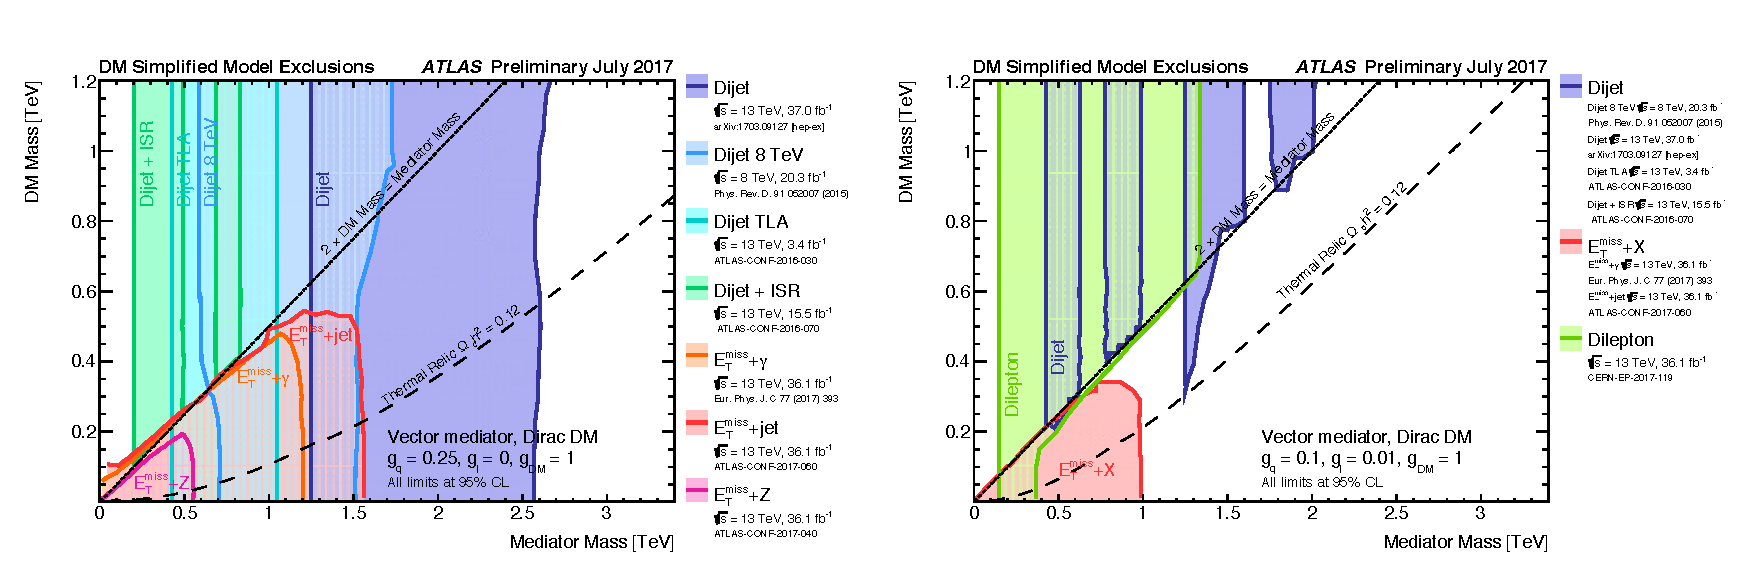
\includegraphics[width=\textwidth]{figures/SummaryPlotsMassMass.pdf}\caption{
Regions in dark matter mass--\Zprime mediator mass excluded at 95\% CL by a selection of ATLAS dark matter searches for two coupling scenarios. Dashed curves labeled "thermal relic" indicate combinations of dark matter and mediator mass that are consistent with a dark matter density of $\omega_c = 0.12 h^2$ and a standard thermal history, as computed in MadDM for this model~\cite{Backovic:2015cra}. The dotted curve indicates the kinematic threshold where the mediator can decay on-shell into dark matter. }
%\gdm=1.0  \gq=0.25universal to all flavors, and a lepton coupling gl set to zero. This choice of couplings corresponds to the "V1" scenario in arXiv:1703.05703. Leptonic decays are absent at tree level. The results use 13 TeV data except for Phys. Rev. D91 052007 (2015). The exclusions from the ATLAS dijet searches are derived from the limits provided on Gaussian-shaped resonances following the procedure recommended by ATLAS in Appendix A of Phys. Rev. D91 052007 (2015) and in arXiv:1703.09127. Small fluctuations in the contour are a product of the dijet reinterpretation scheme. 
%To the left of the curve, annihilation processes described by the simplified model deplete ?c below 0.12 h2. A dotted curve indicates the kinematic threshold where the mediator can decay on-shell into dark matter. The exclusion regions, relic density contours, and unitarity curve are not applicable to other choices of coupling values or model.
\label{fig:sensitivityComparison}
\end{figure}


%It is important to note that generic searches for new two-body resonances are by design sensitive to a broad range of theoretical benchmarks, 
%and as such they alone can offer little information on whether a discovery would imply in terms of invisible particles mediators.

%- narrate coupling dependence
%- point out that when visible searches more specifically target the mediator, and when the invisible particle cannot be produced because too heavy, they are more powerful than generic searches
%- pitfalls: they can't go as low in mMed or m invisible as invisible searches (that only uses more boosted MET)
%-- one cannot generalize about DM from a single simplified model, different production mechanism
%-- the interaction is ruled out for a particular DM mass

Thus, the relative sensitivity of visible and invisible searches is a model- and coupling-dependent statement.
One advantage of searches for invisible particles is their sensitivity to models with very light mediators ($<$50 GeV) and light \mdm, since the reach of dijet and dilepton searches to low-mass resonances is still ultimately limited by data taking constraints. 
%Visearches that more specifically target the mediator are more constraining than their invisible counterparts, in particular if the invisible particle is heavy and cannot be produced at the collider. 
%Invisible particle searches however would dominate whenever the 
%for invisible particles only dominate if the coupling to invisible particles is much larger than the coupling to quarks, and even then reducing \gq reduces the LHC production cross-section and therefore the overall sensitivity of \MET+X searches. When visible searches 
%In absence of a signal and within a specific model scenario, searches for mediator particle with visible decays provide constraints that are complementary to those of searches for invisible particles, in particular in the off-shell region 2\mdm $>$ \mmed where the mediator cannot decay to invisible particles directly but can still decay into much lighter SM particles such as leptons and quarks. 

%[redundancy check?]
%We finally remark again that none of these results rule out invisible particles with a given mass; they rule out {\it interactions} with invisible particles of that mass.

%- pitfalls: they can't go as low in mMed or m invisible as invisible searches (that only uses more boosted MET)
%-- one cannot generalize about DM from a single simplified model, different production mechanism
%-- the interaction is ruled out for a particular DM mass

%Mention why we plot things in the mass-mass plane. 
%A sketch of the comparison of the sensitivity of searches for visible decays of vector and axial vector mediator models, and invisible particles 
%in the \minvisible particles vs \mmed plane is shown in Fig.~\ref{fig:sensitivityComparison}, fixing the couplings. The choice of plane and the scenarios chosen follow the choices of the Dark Matter Working Group~\cite{Albert:2017onk}, to illustrate the complementarity of different LHC searches for $s-$channel-mediated model of invisible particles and to convey the message that the sensitivity of LHC searches to simplified models of invisible particles depends both on model choice and parameter choice. 
%Mention why mass-mass? Because on-shell/off-shell regions clearly spelled out

%Couplings for vector and axial-vector mediated models 

%results are given in the \mdm particles, \mmed  plane fixing the couplings to \gq=0.25 and \gdm particles=1.0 for vector and axial vector mediated models, \gq=\gdm particles=1.0 for scalar and pseudoscalar models and \gdm particlesq=1.0 for colored scalar models. The simplified models employed by the experimental collaborations are known at NLO~\cite{Neubert:2015fka,Haisch:2013ata,Backovic:2015soa}. 

%- putting things together in a global picture is hard, lots of parameters and so forth
%-- there's a 4D param space even in the simplest models

%CD: if we want coupling-mass, we could show the plots in the figs dir: SummaryPlotsCouplingMass.pdf

%In case sample figure with different scenarios as an example
%\begin{figure}[!htpb]
%\includegraphics[width=\textwidth]{figures/invisible particlesSummary.png}
%\caption{Illustrative examples of the comparison of the sensitivity of searches for visible and invisible mediators in the \minvisible particles-\mmed plane, for different coupling scenarios. No actual data has been used, but experimental observations have been used as inspiration for the figure. From~\cite{AnotherWikipedia}.}
%\label{fig:sensitivityComparison}
%\end{figure}

%It would be nice to make tables of lowest mediator/invisible particles searches+refs for 100 GeV invisible particles mass,
%as a poor-person approximation of a summary plot we can't make because ATLAS data not public. 

%%%SUMMARY TABLE FOR MONOX SEARCHES: descoped, unless we just want a list of references of all the searches which may be useful but obsoletes early
%\begin{table}[h]
\tabcolsep7.5pt
\caption{Summary of searches for BSM mediators at the LHC}
\label{tab:BSMSearchesSummary}
\begin{center}
\begin{tabular}{@{}l|c|c|c|c@{}}
\hline
Signature & Model& \mmed limit & \mdm limit  & Cit.\\
 &  & (\mdm=100 GeV) & (\mmed=100 GeV)  &  \\
%{(}units)$^{\rm a}$ &Head 2 &Head 3 &Head 4 &{(}units)\\
\hline
Jets+\MET & $s-$channel, AV$^{\rm a}$ & Column3 & Column4 & \cite{Sirunyan:2017jix,Aaboud:2017phn} \\
Jets+\MET & $s-$channel, V$^{\rm a}$ & Column3 & Column4 & \cite{Sirunyan:2017jix,Aaboud:2017phn} \\
Jets+\MET & colored scalar & Column3 & Column4 & \cite{Sirunyan:2017jix,Aaboud:2017phn} \\
Photon+\MET & Column 2 & Column3 & Column4 & Column\\
W,Z (had)+\MET 1 & Column 2 & Column3 & Column4 &Column\\
W,Z (lep)+\MET 1 & Column 2 & Column3 & Column4 &Column\\
Higgs+\MET &Column 2 & Column3 & Column4 &Column\\
\hline
\end{tabular}
\end{center}
%\begin{tabnote}
$^{\rm a}$ Coupling values: \gq=0.25, \gdm=1.0; $^{\rm b}$second table footnote.
%\end{tabnote}
\end{table}



